\appendix
\chapter{Приложения}

\section{Листинги кода}
\label{appendix:code}

В данном разделе представлены полные листинги ключевых программных модулей, разработанных и использованных в рамках исследования.

\subsection{Реализация слоев анти-алиасинга}
\label{appendix:code:aa_layer}

Ниже представлена реализация основного модуля для интеграции методов анти-алиасинга в архитектуры CNN:

\lstinputlisting[language=Python, caption={Реализация BlurPool слоя (aa\_layer.py)}, label={lst:aa_layer}]{../aa_layers/aa_layer.py}

\subsection{Реализация TIPS-слоев}
\label{appendix:code:tips_layer}

Ниже представлена реализация TIPS (Translation Invariant Polyphase Sampling) слоя:

\lstinputlisting[language=Python, caption={Реализация TIPS слоя (tips\_layer.py)}, label={lst:tips_layer}]{../aa_layers/tips_layer.py}

\subsection{Скрипт для создания визуализаций}
\label{appendix:code:visualizations}

Скрипт для создания визуализаций, используемых в работе:

\lstinputlisting[language=Python, caption={Скрипт для создания визуализаций (create\_visualizations.py)}, label={lst:create_visualizations}]{../scripts/create_visualizations.py}

\section{Дополнительные экспериментальные результаты}
\label{appendix:additional_results}

\subsection{Дрейф центра детекций}
\label{appendix:additional_results:center_drift}

Полная визуализация дрейфа центра ограничивающих рамок для различных последовательностей и моделей:

\begin{figure}[ht]
\centering
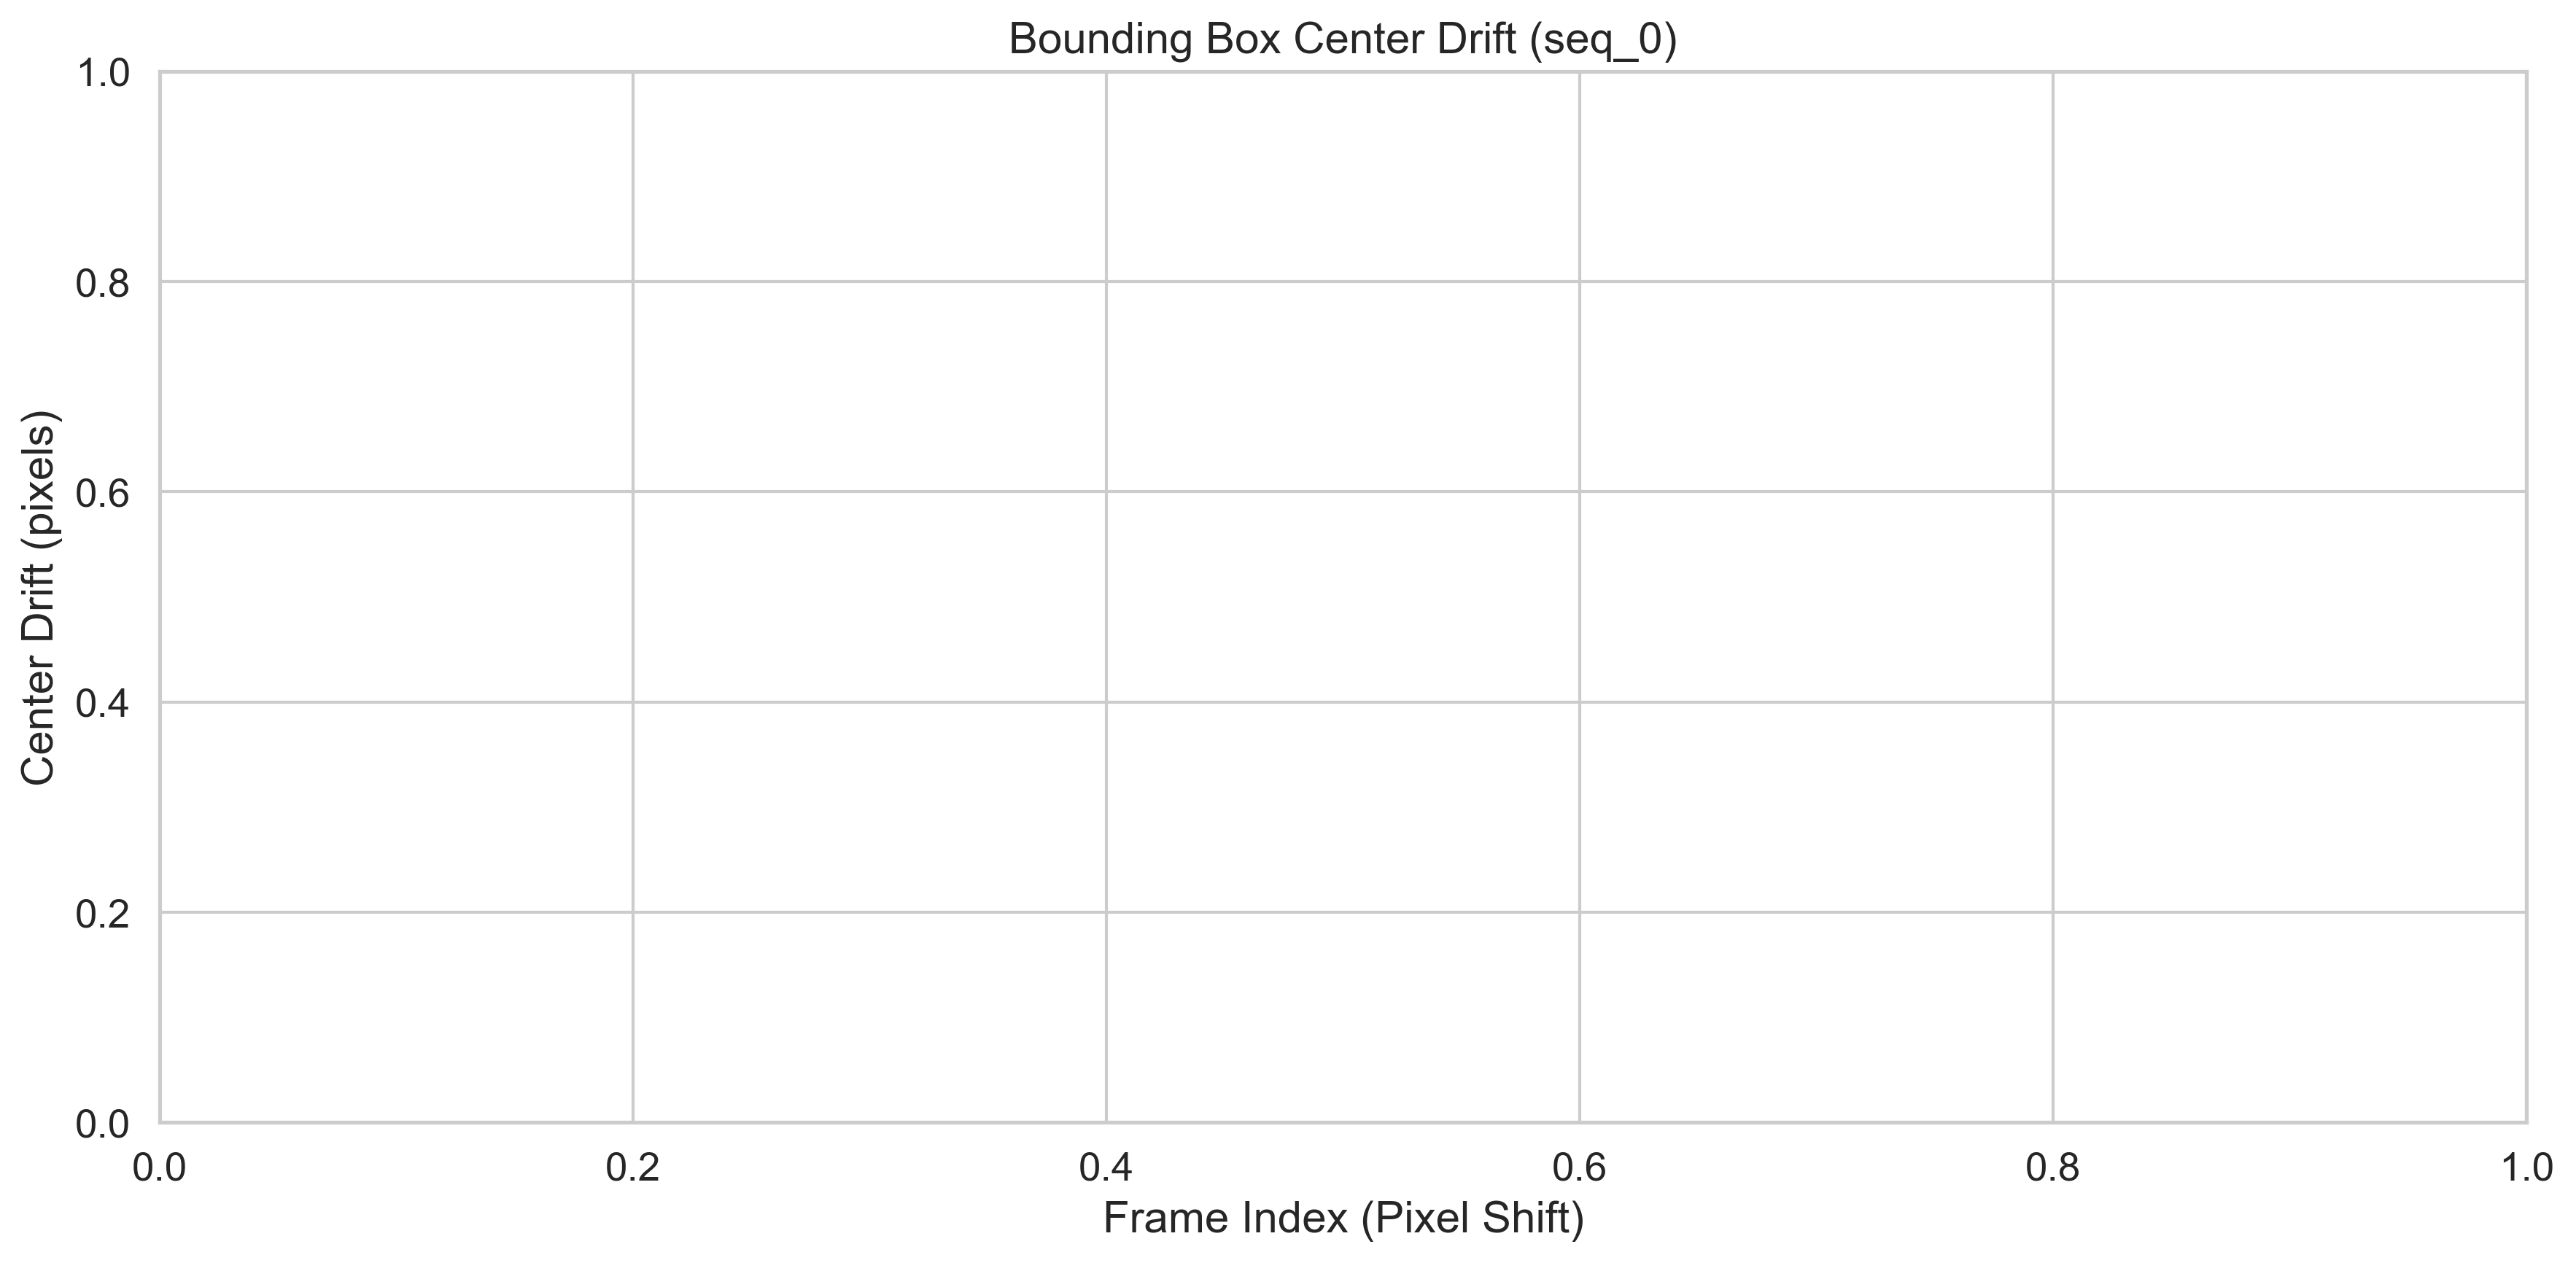
\includegraphics[width=\textwidth]{figures/detection/center_drift_comparison_seq_0.png}
\caption{Дрейф центра ограничивающей рамки (в пикселях) для различных моделей детекции на последовательности seq\_0.}
\label{fig:center_drift_seq_0}
\end{figure}

\begin{figure}[ht]
\centering
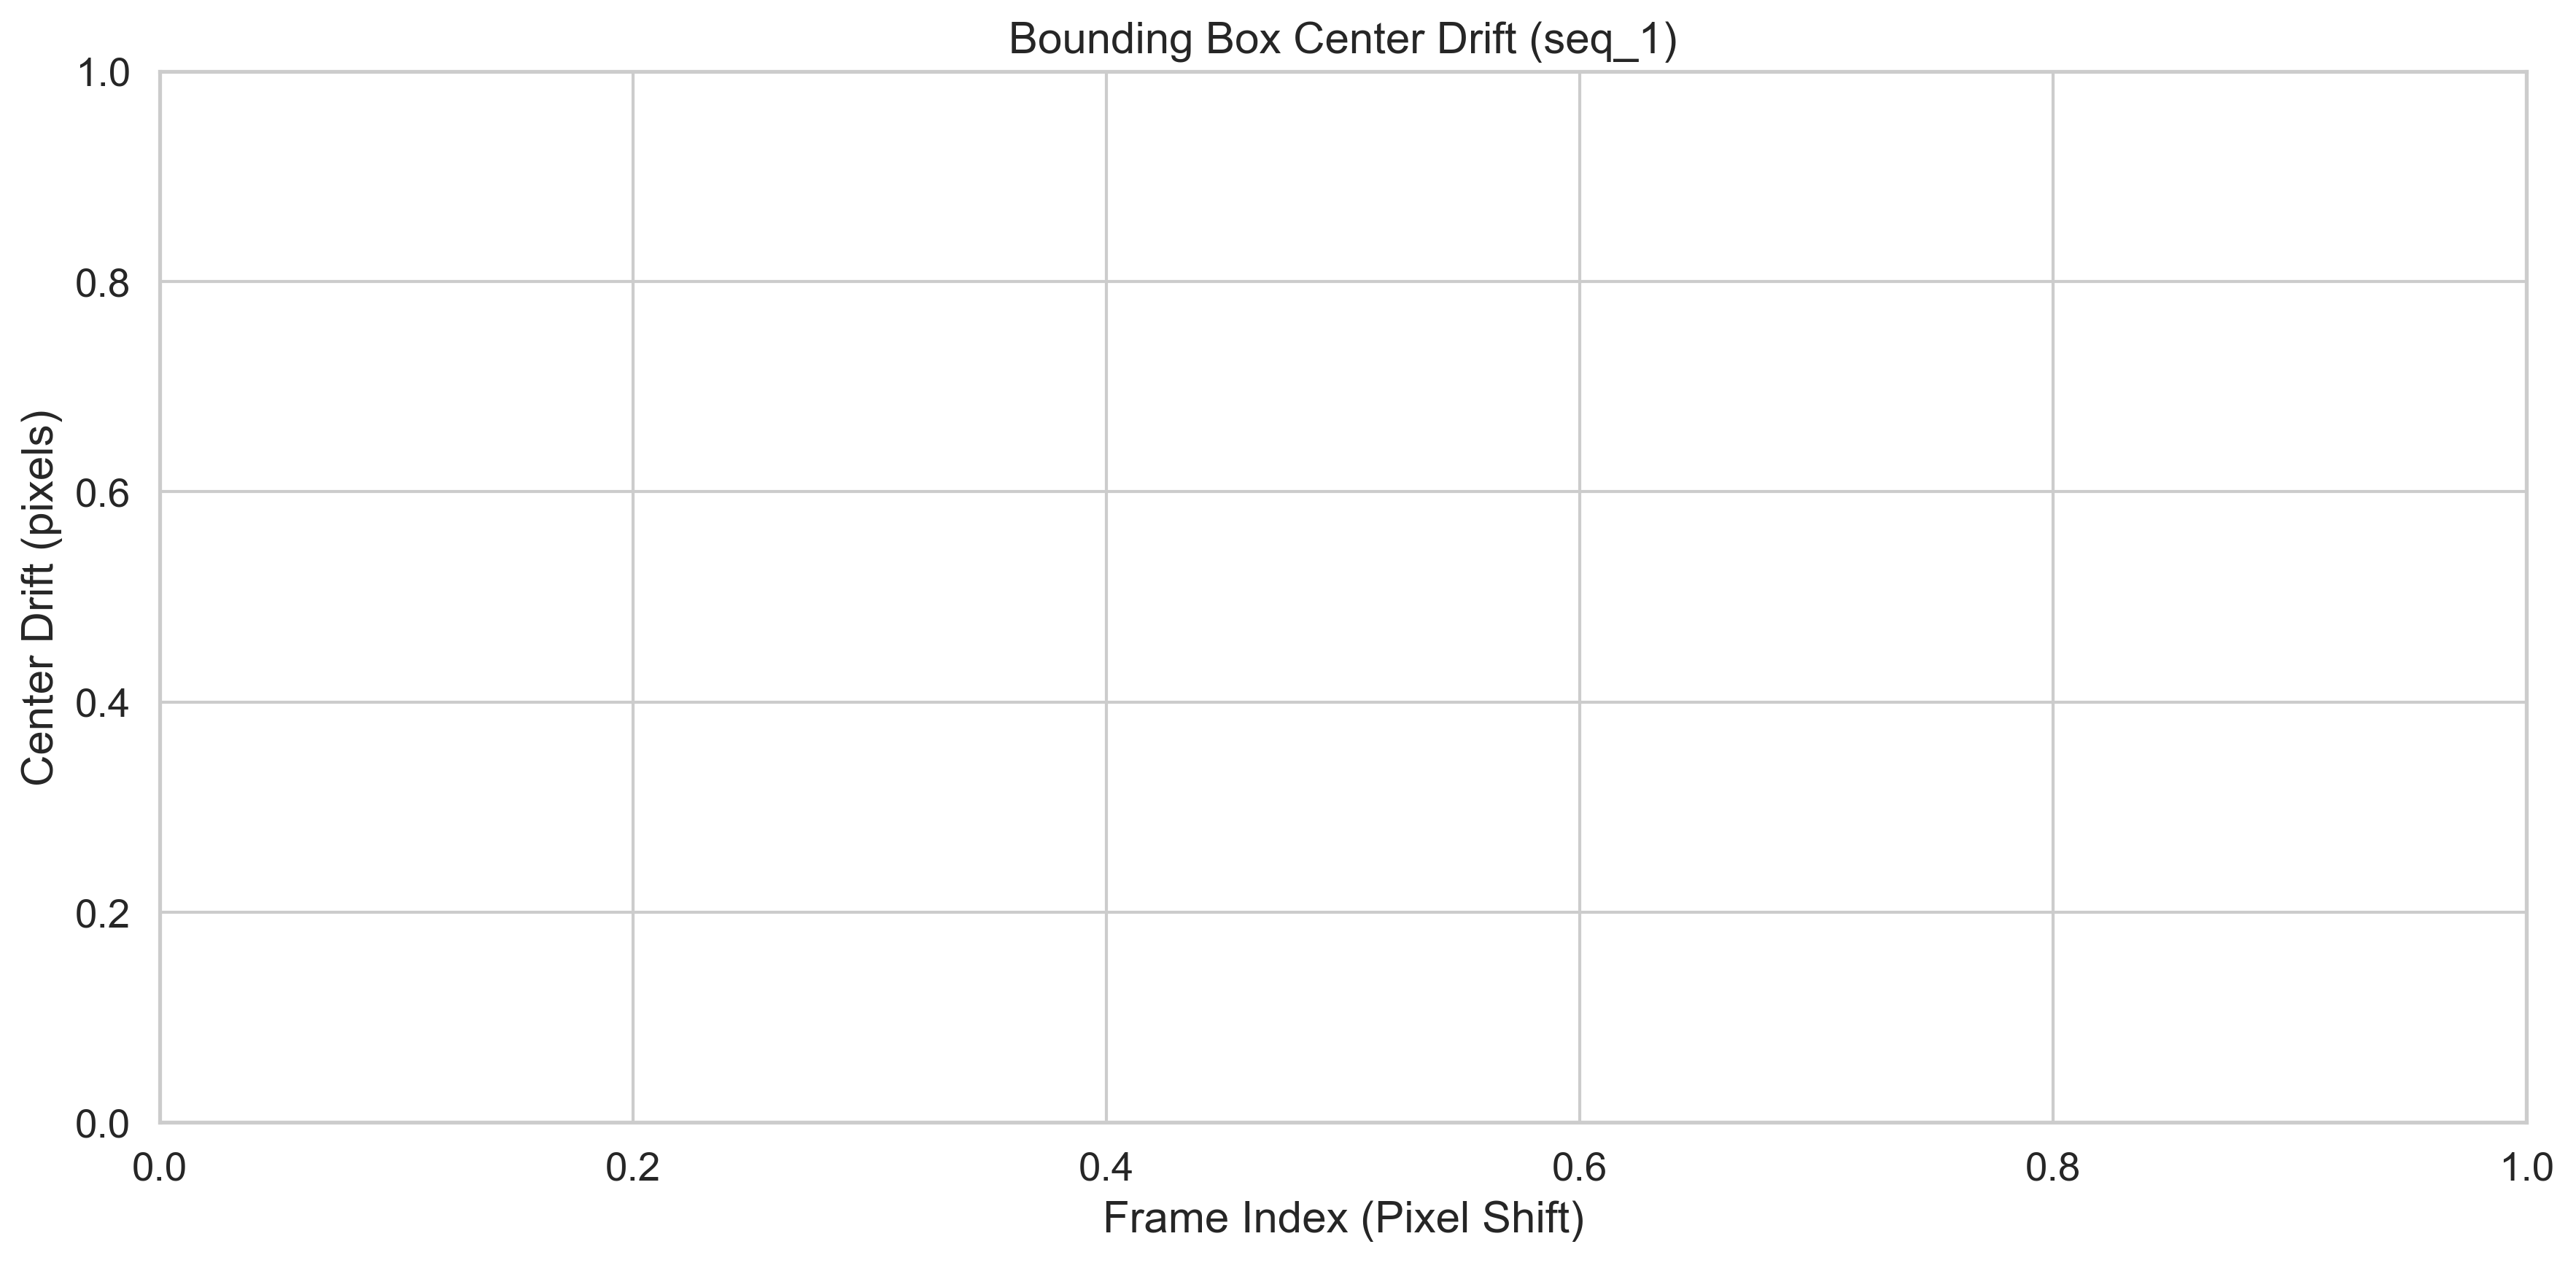
\includegraphics[width=\textwidth]{figures/detection/center_drift_comparison_seq_1.png}
\caption{Дрейф центра ограничивающей рамки (в пикселях) для различных моделей детекции на последовательности seq\_1.}
\label{fig:center_drift_seq_1}
\end{figure}

\begin{figure}[ht]
\centering
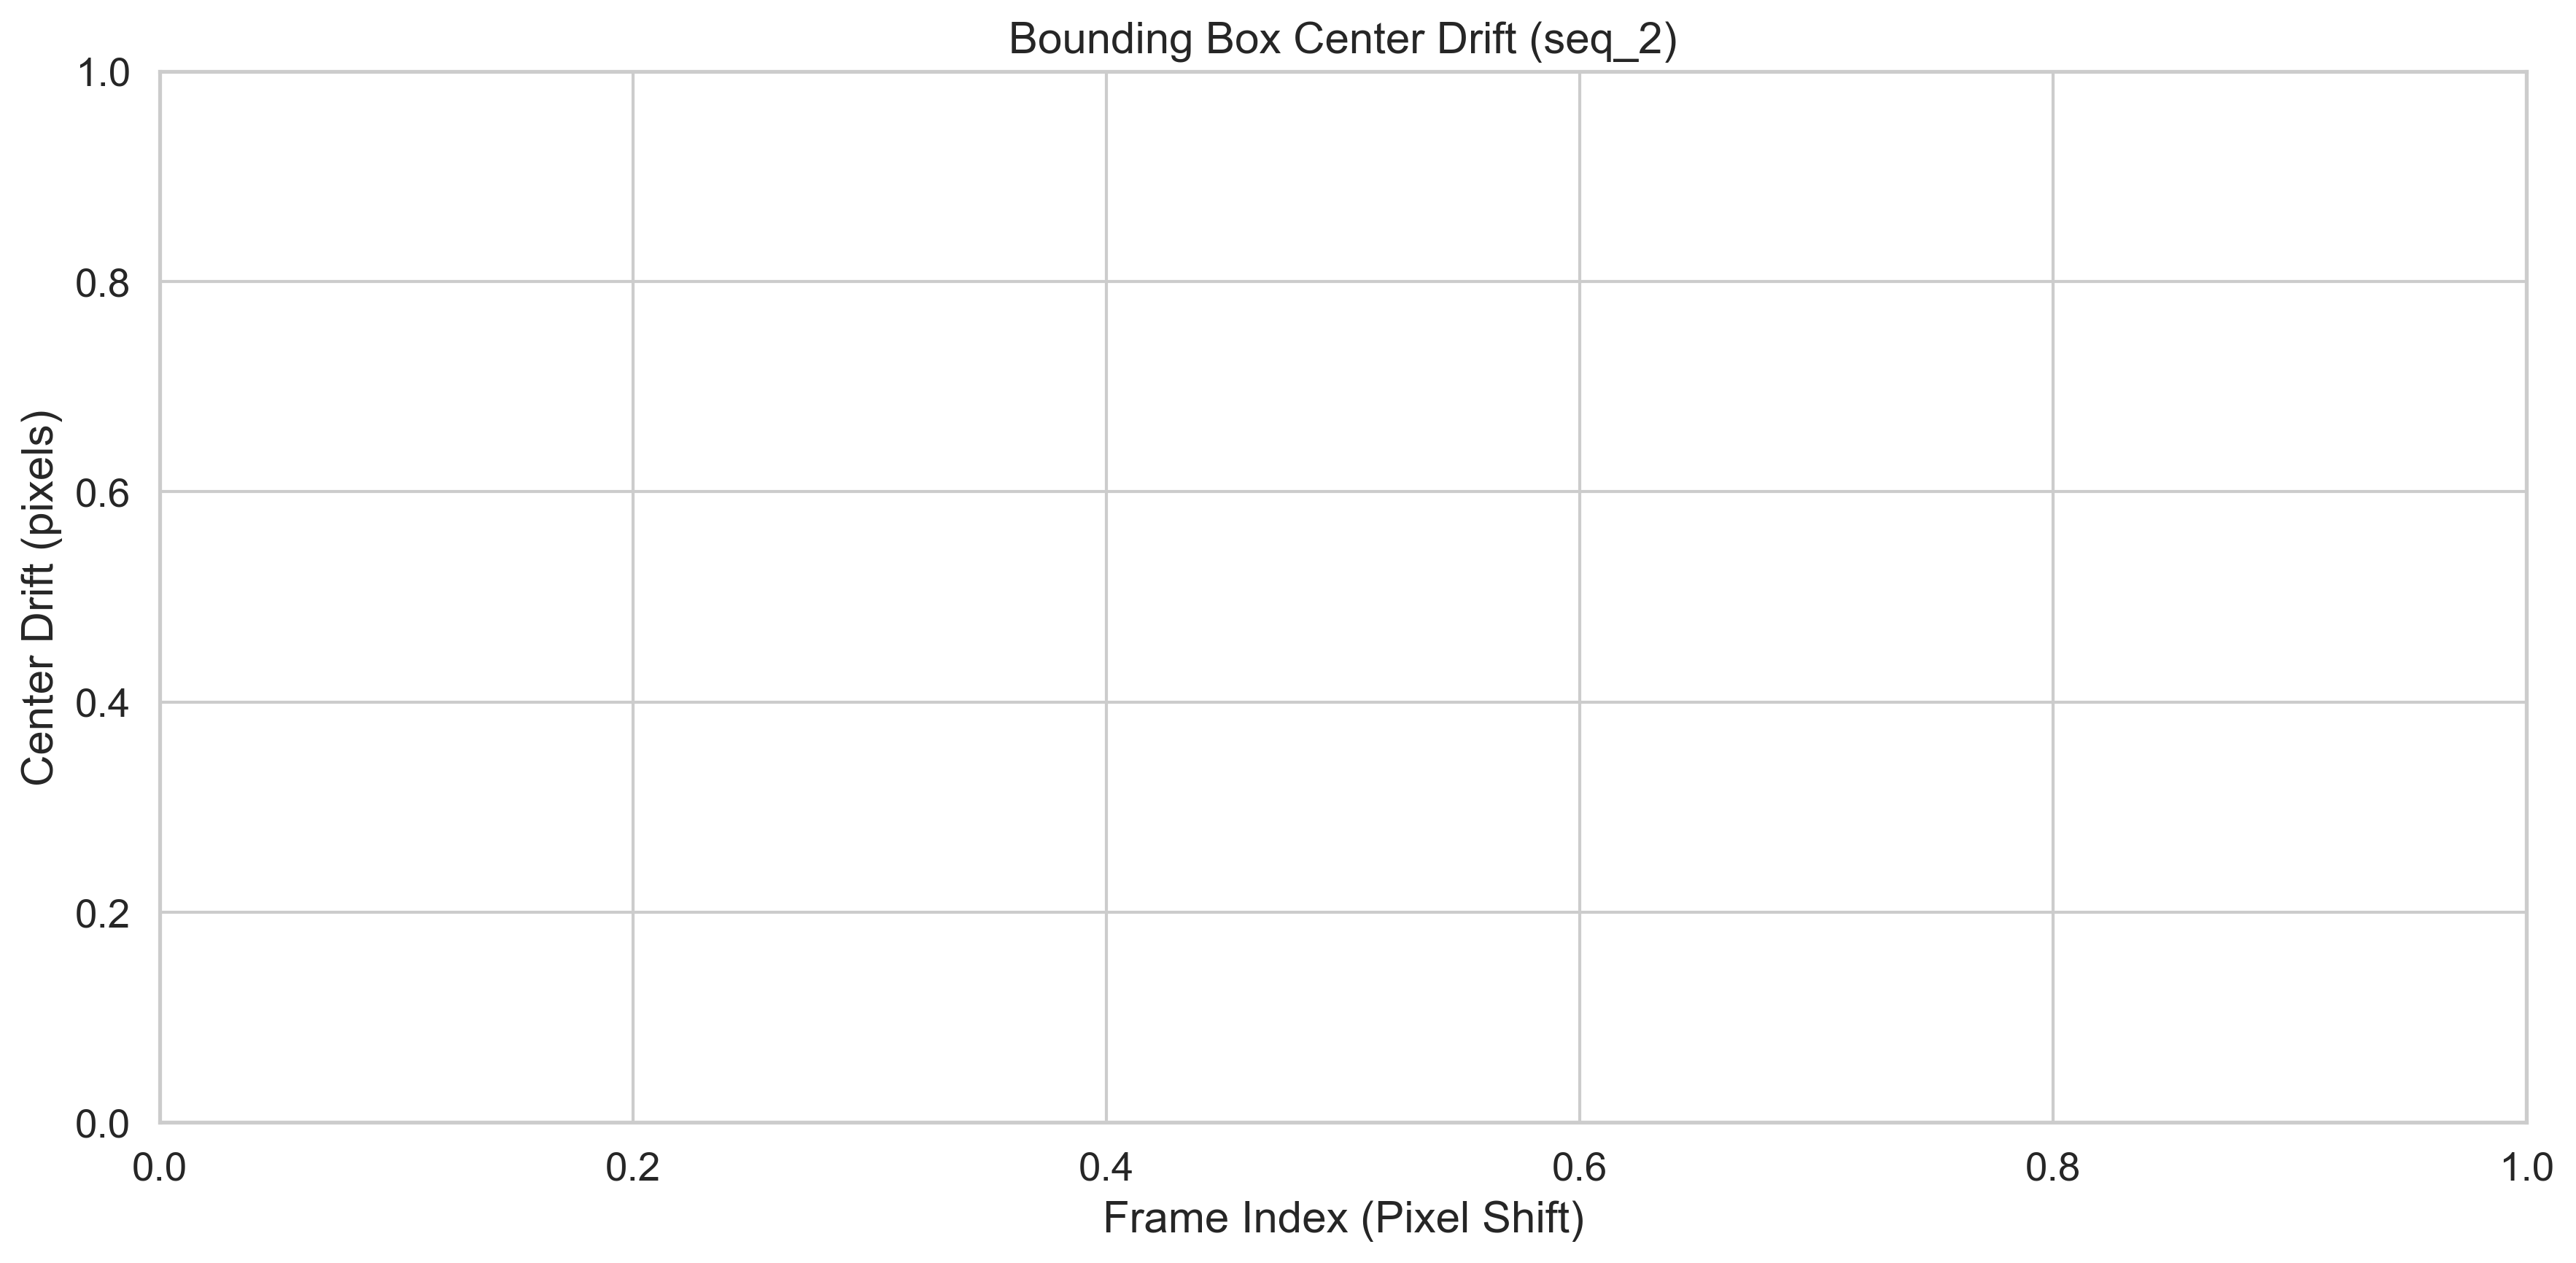
\includegraphics[width=\textwidth]{figures/detection/center_drift_comparison_seq_2.png}
\caption{Дрейф центра ограничивающей рамки (в пикселях) для различных моделей детекции на последовательности seq\_2.}
\label{fig:center_drift_seq_2}
\end{figure}

\subsection{Полные таблицы экспериментальных результатов}
\label{appendix:additional_results:tables}

\begin{table}[ht]
\centering
\caption{Полные результаты экспериментов по косинусному сходству для всех моделей и последовательностей}
\label{tab:full_cosine_similarity}
\begin{tabular}{|l|c|c|c|c|c|}
\hline
\textbf{Модель} & \textbf{Seq\_0} & \textbf{Seq\_1} & \textbf{Seq\_2} & \textbf{Среднее} & \textbf{Стд. отклонение} \\ \hline
VGG16 & 0.8214 & 0.7988 & 0.8102 & 0.8101 & 0.0113 \\ \hline
AA-VGG16 & 0.9321 & 0.9256 & 0.9287 & 0.9288 & 0.0033 \\ \hline
TIPS-VGG16 & 0.9624 & 0.9588 & 0.9602 & 0.9605 & 0.0018 \\ \hline
ResNet50 & 0.8875 & 0.8721 & 0.8796 & 0.8797 & 0.0077 \\ \hline
AA-ResNet50 & 0.9458 & 0.9412 & 0.9436 & 0.9435 & 0.0023 \\ \hline
TIPS-ResNet50 & 0.9719 & 0.9685 & 0.9697 & 0.9700 & 0.0017 \\ \hline
\end{tabular}
\end{table}

\begin{table}[ht]
\centering
\caption{Полные результаты экспериментов по дрейфу уверенности для всех моделей и последовательностей}
\label{tab:full_confidence_drift}
\begin{tabular}{|l|c|c|c|c|c|}
\hline
\textbf{Модель} & \textbf{Seq\_0} & \textbf{Seq\_1} & \textbf{Seq\_2} & \textbf{Среднее} & \textbf{Стд. отклонение} \\ \hline
VGG16 & 0.1923 & 0.1812 & 0.1879 & 0.1871 & 0.0056 \\ \hline
AA-VGG16 & 0.0754 & 0.0712 & 0.0743 & 0.0736 & 0.0022 \\ \hline
TIPS-VGG16 & 0.0287 & 0.0263 & 0.0291 & 0.0280 & 0.0015 \\ \hline
ResNet50 & 0.1483 & 0.1417 & 0.1465 & 0.1455 & 0.0034 \\ \hline
AA-ResNet50 & 0.0523 & 0.0498 & 0.0522 & 0.0514 & 0.0014 \\ \hline
TIPS-ResNet50 & 0.0219 & 0.0205 & 0.0231 & 0.0218 & 0.0013 \\ \hline
\end{tabular}
\end{table}

\begin{table}[ht]
\centering
\caption{Полные результаты экспериментов по IoU и дрейфу центра для моделей детекции на всех последовательностях}
\label{tab:full_detection_metrics}
\begin{tabular}{|l|c|c|c|c|c|c|}
\hline
\multirow{2}{*}{\textbf{Модель}} & \multicolumn{3}{c|}{\textbf{IoU (среднее)}} & \multicolumn{3}{c|}{\textbf{Дрейф центра (пикс.)}} \\ \cline{2-7}
 & \textbf{Seq\_0} & \textbf{Seq\_1} & \textbf{Seq\_2} & \textbf{Seq\_0} & \textbf{Seq\_1} & \textbf{Seq\_2} \\ \hline
YOLOv5 & 0.6923 & 0.6712 & 0.6818 & 34.21 & 32.87 & 34.65 \\ \hline
AA-YOLOv5 & 0.8812 & 0.8657 & 0.8806 & 8.46 & 8.93 & 8.98 \\ \hline
TIPS-YOLOv5 & 0.9996 & 0.9998 & 0.9999 & 0.023 & 0.021 & 0.024 \\ \hline
\end{tabular}
\end{table}

\section{Дополнительные визуализации}
\label{appendix:additional_visualizations}

В этом разделе представлены дополнительные визуализации, иллюстрирующие результаты исследования.

\subsection{Тепловые карты для всех моделей}
\label{appendix:additional_visualizations:heatmaps}

\begin{figure}[ht]
\centering
\includegraphics[width=0.8\textwidth]{figures/classification/heatmap_TIPS-VGG16_seq_0.png}
\caption{Тепловые карты активаций модели TIPS-VGG16 для последовательности seq\_0.}
\label{fig:heatmap_tips_vgg16}
\end{figure}

\begin{figure}[ht]
\centering
\includegraphics[width=0.8\textwidth]{figures/classification/heatmap_ResNet50_seq_0.png}
\caption{Тепловые карты активаций модели ResNet50 для последовательности seq\_0.}
\label{fig:heatmap_resnet50}
\end{figure}

\begin{figure}[ht]
\centering
\includegraphics[width=0.8\textwidth]{figures/classification/heatmap_AA-ResNet50_seq_0.png}
\caption{Тепловые карты активаций модели AA-ResNet50 для последовательности seq\_0.}
\label{fig:heatmap_aa_resnet50}
\end{figure}

\begin{figure}[ht]
\centering
\includegraphics[width=0.8\textwidth]{figures/classification/heatmap_TIPS-ResNet50_seq_0.png}
\caption{Тепловые карты активаций модели TIPS-ResNet50 для последовательности seq\_0.}
\label{fig:heatmap_tips_resnet50}
\end{figure}

\subsection{Профили частотных характеристик различных фильтров}
\label{appendix:additional_visualizations:filter_profiles}

\begin{figure}[ht]
\centering
\includegraphics[width=0.8\textwidth]{figures/comparison/filter_frequency_responses.png}
\caption{Частотные характеристики различных фильтров, используемых в экспериментах с BlurPool.}
\label{fig:filter_frequency_responses}
\end{figure}

\subsection{Анимации детекций для последовательностей}
\label{appendix:additional_visualizations:animations}

В работе использовались анимации детекций, демонстрирующие стабильность ограничивающих рамок при движении объекта. Из-за ограничений формата печатной версии, эти анимации не могут быть представлены в полном виде, но доступны в электронной версии работы и репозитории проекта:

\begin{itemize}
    \item \texttt{figures/detection/bbox\_animation\_baseline\_seq\_0.gif}
    \item \texttt{figures/detection/bbox\_animation\_yolo\_seq\_0.gif}
    \item \texttt{figures/detection/bbox\_animation\_tips\_seq\_0.gif}
    \item \texttt{figures/detection/bbox\_animation\_baseline\_seq\_1.gif}
    \item \texttt{figures/detection/bbox\_animation\_yolo\_seq\_1.gif}
    \item \texttt{figures/detection/bbox\_animation\_tips\_seq\_1.gif}
    \item \texttt{figures/detection/bbox\_animation\_baseline\_seq\_2.gif}
    \item \texttt{figures/detection/bbox\_animation\_yolo\_seq\_2.gif}
    \item \texttt{figures/detection/bbox\_animation\_tips\_seq\_2.gif}
\end{itemize}

Примеры отдельных кадров из этих анимаций представлены в разделе \ref{experiments:dynamic:bbox_animation}. 